\documentclass{article}
\usepackage[utf8]{inputenc}
\usepackage{graphicx}
\usepackage[margin=1in]{geometry}
\usepackage{hyperref}
\usepackage{natbib}



\title{PASIPHAE - Observation Planner Software}
\author{John A. Kypriotakis, Poorva Bhalerao, Siddharth Maharana}
\date{\today}

\begin{document}

\maketitle

\section{Introduction}
The purpose of this document is to introduce the PASIPHAE collaboration to the necessity, the operation principles, the development and the timeline of the observation planner software that will accompany the survey.

\section{Description}
The observation planner algorithm of PASIPHAE will be an almost entirely independent system that will handle the scheduling of observations over the complete duration of the survey, at both observing sites. Its fundamental role is to optimize the observing strategy in terms of time and other costly resources. The algorithm will choose the ‘best’ field to be observed by the telescope at a particular point of time and forward this decision to the telescope control pipeline. This technique surpasses most previously used surveying strategies such as the drift mode of the ALFALFA survey [\cite{Giovanelli2005}] and other multiple-pass strategies as it will continously strive to eliminate capturing of bad science images. 

\section{Operation principle}
The core of the algorithm will be a merit function with a set of static and dynamic input variables. The value of this merit function will decide the priority of a field to be observed and an output analogous to a heat map will be generated based on the priority for each field.

\section{Target features}
The algorithm must have the following features in order to perform as expected:
\begin{enumerate}
\item Correct balance between the merit terms, in order to accurately estimate the merit of each candidate field.
\item Time-efficiency in calculation of the merit function.
\item Self-consistency and good grouping of fields to be observed in coherent patches.
\item Ability to handle the unexpected.
\end{enumerate}

\clearpage
\section{The Base Algorithm}
The observation planner will comprise of three main abstract components - the preample, the minimizer and the announcer, as presented in figure \ref{fig:baseflow}
\begin{figure}[!ht]
\centering
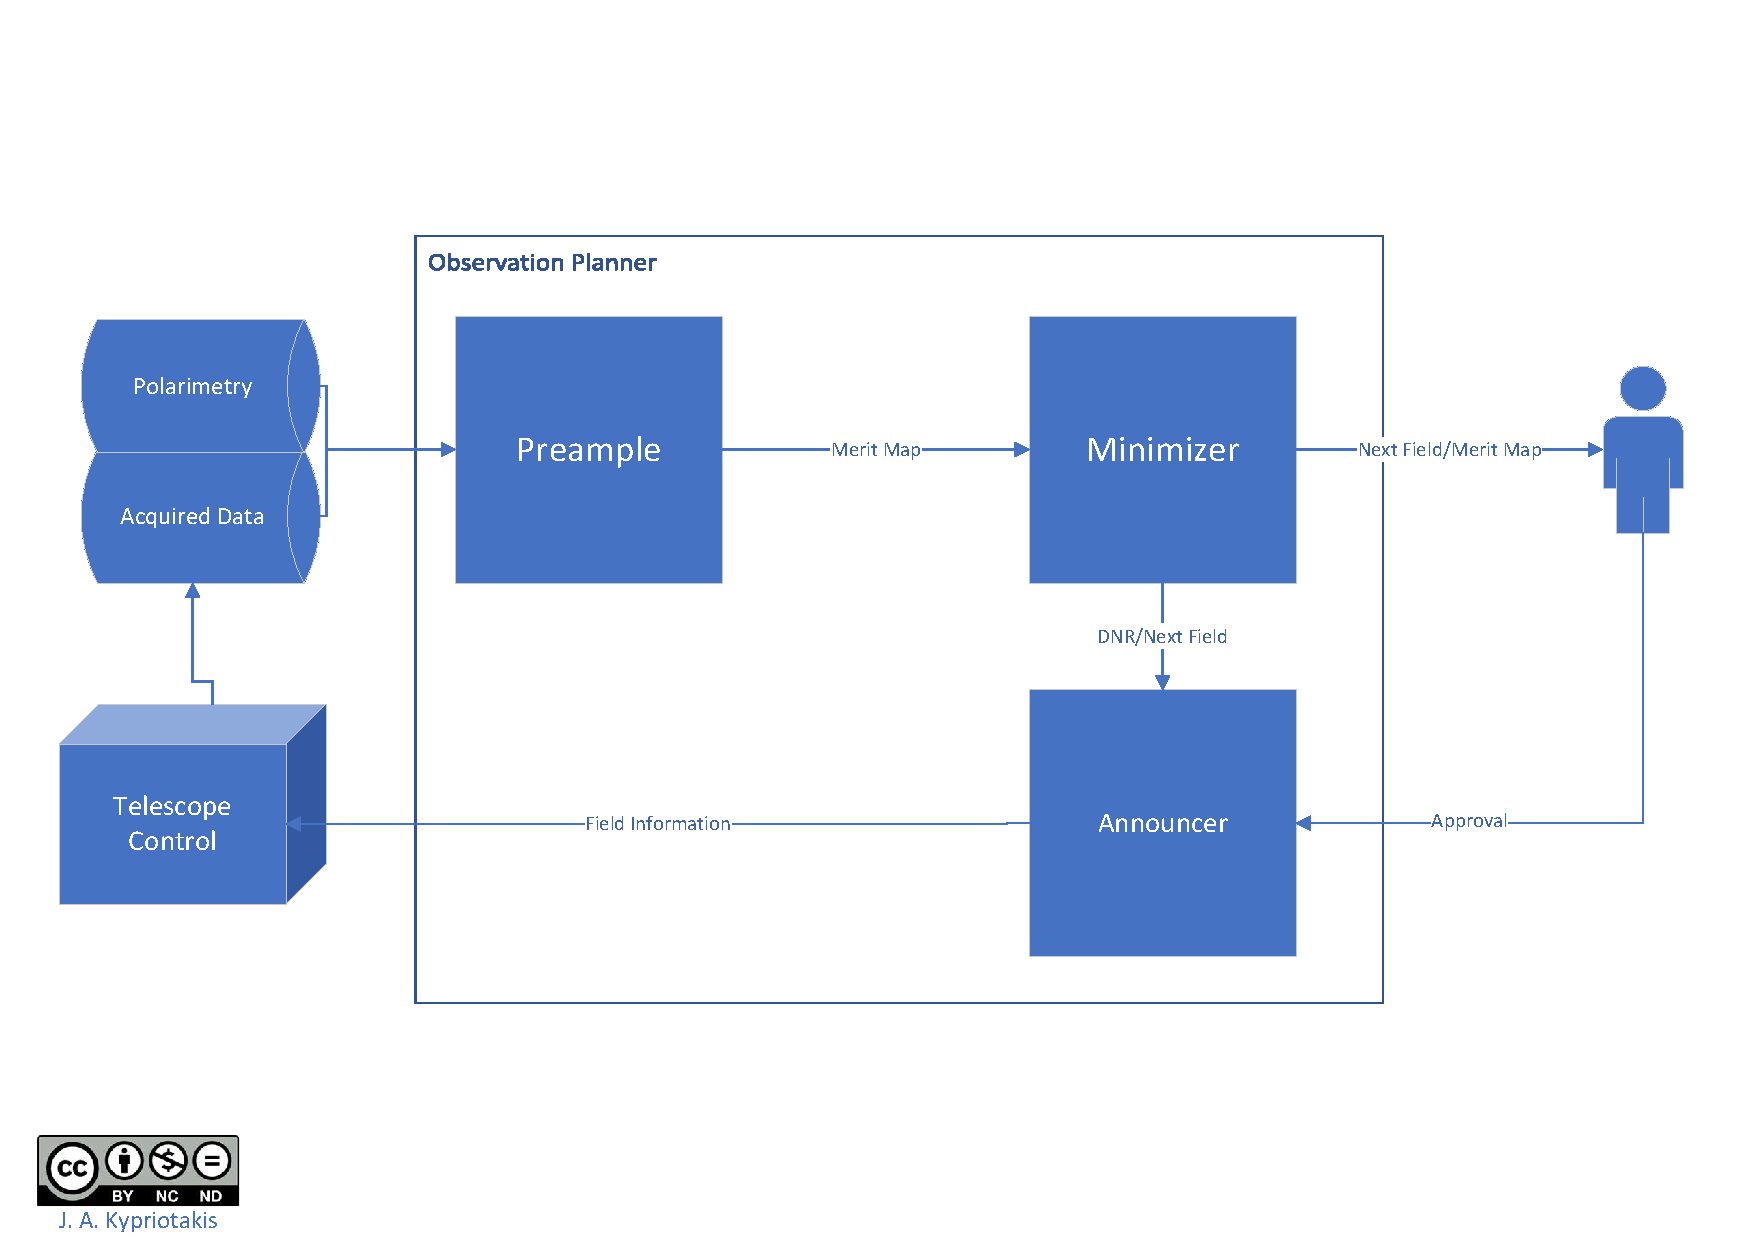
\includegraphics[width=\linewidth]{Base_new.pdf}
\caption{The base flow chart of the observation planning algorithm.}
\label{fig:baseflow}
\end{figure}

\subsection{Preample}
The preample handles a set of inputs (which are mentioned in section \ref{sec:ins}) from various sources for each component of the merit function, computes the value of the merit function and passes a merit map to the minimizer.

\subsection{Minimizer}
The minimizer then looks for the field with the highest merit i.e. the field having the highest priority (taking into account the coherency of the observed and candidate fields) and sends an approval request to the telescope operator. The operator then approves this decision and the approval is passed on to the announcer. In case the operator does not respond, or has set the algorithm to full-auto mode, the minimizer directly invokes the announcer. 

\subsection{Announcer}
The announcer accepts the chosen field and sends the corresponding pointing information to the Telescope Control. The acquired data, as one of the input modules, will in turn be fed back to the preample as an input to construct an updated metric map.

\section{Input Parameters}\label{sec:ins}
The set of input parameters can be divided into: static inputs, dynamic inputs and user assisted inputs. A brief description of each of the inputs is provided below.

\subsection{Static Inputs}
Static inputs are the parameters that we do not expect to change within the span of our survey.
\begin{enumerate}
\item Intended survey coverage: \\
The intended survey coverage of the northern and southern Galactic poles.

\item Earth-bound light contamination: \\
The location, altitude and proximity of potential light contaminants (e.g. city lights, telecommunications antennae, wind turbines).

\item Specifications and limitations of the telescope, instrument and dome:
\begin{enumerate}
	\item Field size
	\item Slew speed
	\item Instrument sensitivity
	\item Instrument readout time
	\item Expected observing season
\end{enumerate}
\end{enumerate}

\subsection{Dynamic Inputs}
The dynamic inputs are the parameters that we expect to vary with either large or small frequency through the survey period.
\begin{enumerate}
	\item Lunar phase and lunar position (deterministic parameter)\\
	\item Wind \&{} Atmospheric conditions (non-deterministic parameter)\\
	\item Current telescope position (deterministic parameter)\\
	\item Existing image quality (deterministic parameter)\\
	\item Length of exposure (quasi-deterministic parameter)\\
	\item Down time (quasi-deterministic parameter)\\
\end{enumerate}
Deterministic dynamical inputs are those that under all circumstances can be determined beforehand. Quasi-deterministic parameters are those that usually can be determined before the observations actually commence and, if they vary, they do so with prior notice. Non-deterministic parameters will vary without prior notice and are usually not predictable.

\subsection{User Assisted Inputs - High Importance Fields}
Fields with objects of opportunity, transient phenomena and other science-driven goals will be assigned priority by the users.

\section{Merit Function Terms}
The field priorities will be calculated by the merit function. The aforementioned input parameters will be handled by submodules in order to be mathematicized, to be included as terms in this merit function. Mathematizing the input parameters implies quantifying the input factors and expressing their influence as a mathematical expression.

The terms of the merit function will include:

\begin{enumerate}
	\item Slew time (the more time required to slew, the smaller the merit of the field - zero influence to fields with slew time less than the readout time)\\
	\item Weather influence (the larger the influence of the nature elements (face wind, dust, etc.), the smaller the merit of the field)\\
	\item Existing image quality (if the field has been observed before then the priority is reduced, the priority becomes 0 for fields with observed polarimetric $\frac{S}{N}>3$, clustering of fields increases their merit)\\
	\item Required depth (fields with less bright stars, or contaminated by other light sources (moon, city lights etc.) have reduced merit)\\
	\item Custom prioritization (user-prioritized fields have higher merit)
\end{enumerate}

After defining the exact mathematical formulae relating the input parameters to their contribution in the above merit function terms, the terms will be weighted and the total merit function will be constructed. 

\section{Development}
The dev-team of the algorithm is led by J. A. K. (Ph.D. fellow, UoC) and includes S.M. (Senior Ph.D. Research Scholar, IUCAA), P.B. (Undergraduate project student, IUCAA) and Rahul Sanghvi (Undergraduate project student, IUCAA).

\section{Timeline}
The mentioned team will develop the algorithm, attempting to follow the following timeline:

\begin{enumerate}
	\item Development of analytic functions and their corresponding side-modules / Deliverable: side-modules explanatory document, beta of side-modules / Second half of February 2019
	\item Development of the preample, minimizer, announcer and wrapper, testing and proofing of the algorithm / Deliverable: observation planner and its manual / Second half of March 2019
\end{enumerate}

\nocite{*}
\bibliography{biblio}
\bibliographystyle{mnras}

\end{document}
